\documentclass[12pt,letterpaper,titlepage]{article}

\usepackage{fontspec}
\defaultfontfeatures{Mapping=tex-text}
\usepackage{xunicode}
\usepackage{xltxtra}
\usepackage{amsmath}
\usepackage{pdfpages}
\usepackage{amsfonts}
\usepackage{bbold}
\usepackage{amssymb}
\setcounter{secnumdepth}{0}
\usepackage{nameref}
\usepackage{enumitem}
\usepackage{environ}
\usepackage{pgfplots}

\showboxdepth=\maxdimen
\showboxbreadth=\maxdimen


\usepackage{paracol}
\usepackage{wrapfig}
\globalcounter{table}
\globalcounter{figure}
\usepackage{graphicx}
\usepackage[left=1in,right=1in,top=1in,bottom=1in]{geometry}
\graphicspath{{img/}}

\author{Jacob Abel}
\title{	Design \& Simulate 6 Ex1.9
	\\\large ECE2204 CRN:82929
}

\setlength{\parskip}{0.5em}

\begin{document}
\maketitle
\begin{raggedright}

\section{Problem 6.9.a.1: }
\subsection{Design}
Assume that in the pictured circuit that the diode is actually two identical diodes in series $D_1$ and $D_2$ with $D_1$ being closest to the resistor. Determine the mode, diode voltage $V_{D1}$, $V_{D2}$, current $I_{D1}$, $I_{D2}$, and power dissipated by the diode $P_{D1}$, $P_{D2}$ in the circuit below. When determining the mode, assume all diodes are off. Assume  piecewise linear diode parameters for both diodes are $V_\gamma = 0.6V$ and $r_f = 10\Omega$.
\begin{center}
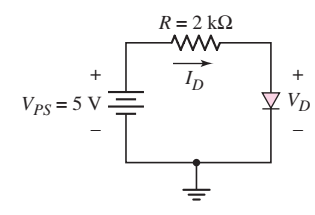
\includegraphics[width=\textwidth, height=9\baselineskip, keepaspectratio=true]{ds1}
\end{center}
\begin{equation}\scalebox{1.25}{
$
V_{D1} = V_{PS} = 5V \implies V_{D1} > V_\gamma \implies \text{Diode 1 is on.}
$
}
\end{equation}
\begin{equation}\scalebox{1.25}{
$
V_{D2} = V_{D1} - V_\gamma = 4.4V \implies V_{D2} > V_\gamma \implies \text{Diode 2 is on.}
$
}
\end{equation}
\begin{equation}\scalebox{1.25}{
$
I_{D1} = I_{D2} = I_D = \frac{V_{PS} - V_{\Sigma\gamma}}{R + r_{\Sigma f}} = \frac{5V - (0.6V + 0.6V)}{2k\Omega + (10\Omega + 10\Omega)} = 1.881mA
$
}
\end{equation}
\begin{align}
V_{D} &= V_\gamma + I_D r_f 
\\ V_{D1} = V_{D2} &= V_\gamma + I_D r_f = 0.6V + 1.881mA \times 10\Omega = 0.619V 
\\ V_{\Sigma D} &= V_{D1} + V_{D2} = 2\times 0.619V = 1.238V
\end{align}
\begin{align}
P_D &= I_D \times V_D
\\ P_{D1} = P_{D2} &= 1.881mA \times 0.619V = 1.164 mW
\\ P_{\Sigma D} = I_D \times V_{\Sigma D} &= 1.881mA \times 1.238V = 2.329 mW
\end{align}

The voltage, current, and power are the same for Diodes 1 and 2. They are $V_D = 0.619V$, $I_D = 1.881mA$, and $P_D = 1.164 mW$. The voltage, current, and power for the diode series are as follows. $V_{\Sigma D} = 1.238V$, $I_{\Sigma D} = I_D = 1.881mA$, and $P_{\Sigma D} = 2.329 mW$.

\subsection{Validation}

\begin{center}
LTSpice Implementation (accurate with $< 1\%$ deviation from design result)
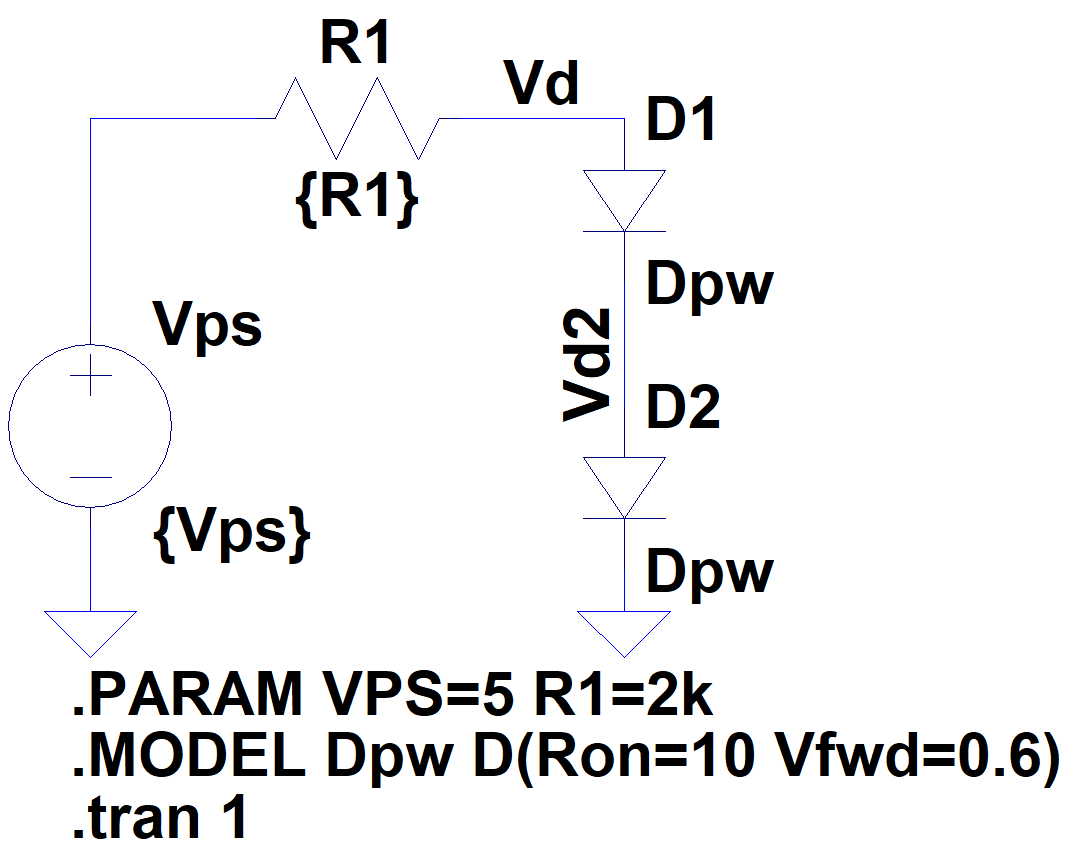
\includegraphics[width=.39\textwidth, height=\textheight, keepaspectratio=true]{ds1b}
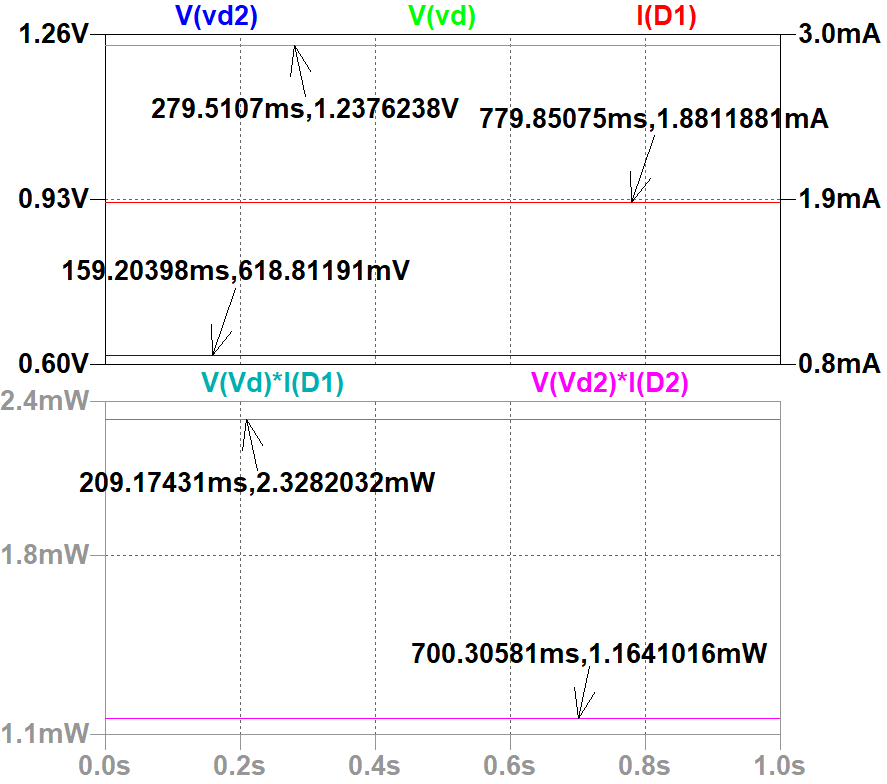
\includegraphics[width=.6\textwidth, height=\textheight, keepaspectratio=true]{ds1c}
\columnratio{0.45}
\begin{paracol}{2}
$Err_{VD} = \frac{|619-618|}{619} = 0.0016 = 0.16\%$
\switchcolumn
$Err_{ID} = \frac{|1.881-1.881|}{1.881} = 0.00 = 0.00\%$
\switchcolumn
$Err_{PD} = \frac{|1.164-1.164|}{1.164} = 0.00 = 0.00\%$
\switchcolumn
$Err_{V\Sigma D} = \frac{|1.238-1.237|}{1.238} = 0.0008 = 0.08\%$
\switchcolumn
$Err_{P\Sigma D} = \frac{|2.329-2.328|}{2.329} = 0.0004 = 0.04\%$
\switchcolumn
$Err_{Avg} = \frac{0.0016 + 0 + 0 + 0.0008 + 0.0004}{5} = 0.056\%$
\end{paracol}
\end{center}

\clearpage
\section{Problem 6.9.b.1: } Derived by merging the problem 1.44 and the circuit for 1.42 and changing the values.
\subsection{Design}
Consider the circuit shown below. Determine the diode currents $I_{D1-D3}$ and voltages $V_{D1-D3}$. The following are the piecewise linear diode parameters for these diodes. $V_\gamma = 0.7V$ and $r_f = 6\Omega$. Assume $V_1 = V_{PS} = 10V$.
\begin{center}
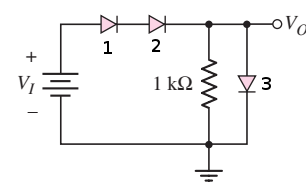
\includegraphics[width=\textwidth, height=7\baselineskip, keepaspectratio=true]{ds2}
\end{center}

\begin{equation}\scalebox{1.25}{
$
V_{D3} = V_{R} \implies V_{PS} = V_{D1} + V_{D2} + V_{D3} = V_{D1} + V_{D2} + V_{R}
$
}
\end{equation}
\begin{equation}\scalebox{1.25}{
$
I_{D1} = I_{D2} = I_{D3} = \frac{V_{PS} - 3\times V_\gamma}{R + 3\times r_f} = \frac{10V - 3\times 0.7V}{0+ 3\times 6\Omega} = 438.9mA
$
}
\end{equation}
\begin{align}
V_{D} &= V_\gamma + I_D r_f 
\\ V_{D1} = V_{D2} = V_{D3} &= V_\gamma + I_{D1} r_f = 0.7V + 438.9mA \times 6\Omega = 3.333V 
\end{align}

\clearpage
\subsection{Validation}

\begin{center}
LTSpice Implementation (accurate with $< 1\%$ deviation from design result)
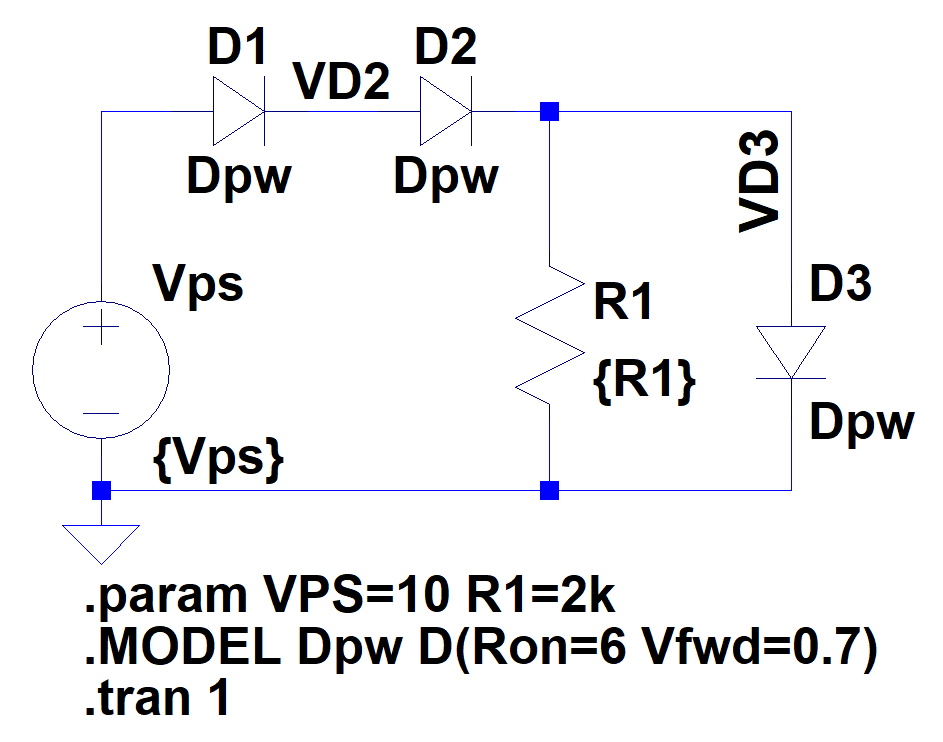
\includegraphics[width=.49\textwidth, height=\textheight, keepaspectratio=true]{ds2b}
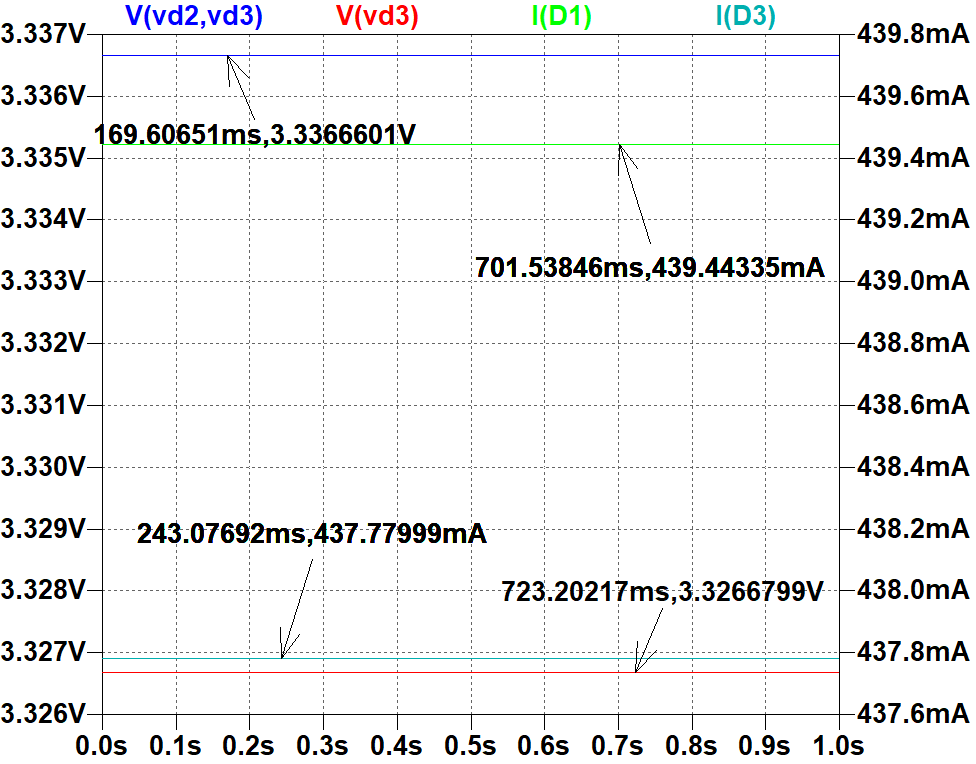
\includegraphics[width=.49\textwidth, height=\textheight, keepaspectratio=true]{ds2c}
\columnratio{0.55}
\begin{paracol}{2}
$Err_{VD1 \& VD2} = \frac{|3.333-3.336|}{3.333} = 0.0009 = 0.09\%$
\switchcolumn
$Err_{VD3} = \frac{|3.333-3.326|}{3.333} = 0.002 = 0.20\%$
\switchcolumn
$Err_{IDI \& ID2} = \frac{|438.9-439.4|}{438.9} = 0.0011 = 0.11\%$
\switchcolumn
$Err_{ID3} = \frac{|438.9-438.7|}{438.9} = 0.0004 = 0.04\%$
\switchcolumn
$Err_{Avg} = \frac{0.09 + 0.20 + 0.11 + 0.04}{4} = 0.11\%$
\end{paracol}
\end{center}

This assignment demonstrates a basic understanding of approximating diode circuits using piecewise linear analysis.

\textit{I have neither given nor received unauthorized assistance on this assignment.}


\end{raggedright}
\end{document}
